\section{Zielsetzung}
\label{sec:Zielsetzung}

\section{Theorie}
\label{sec:Theorie}

Das Geiger-Müller-Zählrohr ist ein Detektor für ionisierende Strahlung. 
Ionisierende Strahlung ist in α-, β- und γ-Strahlung unterteilt. 
α-Strahlung besteht aus Heliumkernen, β-Strahlung aus Elektronen und γ-Strahlung aus Photonen.
Das Geiger-Müller-Zählrohr ist am besten für die Messung von 
α- und γ-Strahlung geeignet. Die Nachweisbarkeit von γ-Strahlung ist klein.
\\
Das Zählrohr besteht aus aus einem Anodendraht und einer Kathodenhülle.
Zwischen Kathode und Anode wird eine Spannung angelegt.
Durch eine dünne Mylarfolie ist das Rohr verschlossen.
Im Inneren befindet sich ein Gasgemisch aus Argon und einem Alkohol.
Durch eintretende Strahlung wird Argon ionisiert. 
Aufgrund das E-Feld im Inneren werden die Gasionen zum Kathodenzylinder und die Elektronen zum Anodendraht hin beschleunigt.
Die freigesetzten Elektronen können auf ihrem Weg zur Kathode in einer Kettenreaktion weitere Ion-Elektron-Paare erzeugen.
Über diesen Prozess wird ein Stromfluss erzeugt, welcher jedoch schnell wieder über den Widerstand im $\si{\m\O}$-Bereich abfällt.
So bald die Ladungsträger wieder abgeflossen sind baut sich das E-Feld im inneren des Zählrohrs wieder auf.
\\
Aufgrund der geringen Stärke der Spannungsimpulse, müssen sie mithilfe eines Versärkers 
für den angeschlossenen Zähler verstärkt werden.
\\
\begin{figure}[h!]
    \label{fig:gm-charakteristik}
    \centering
    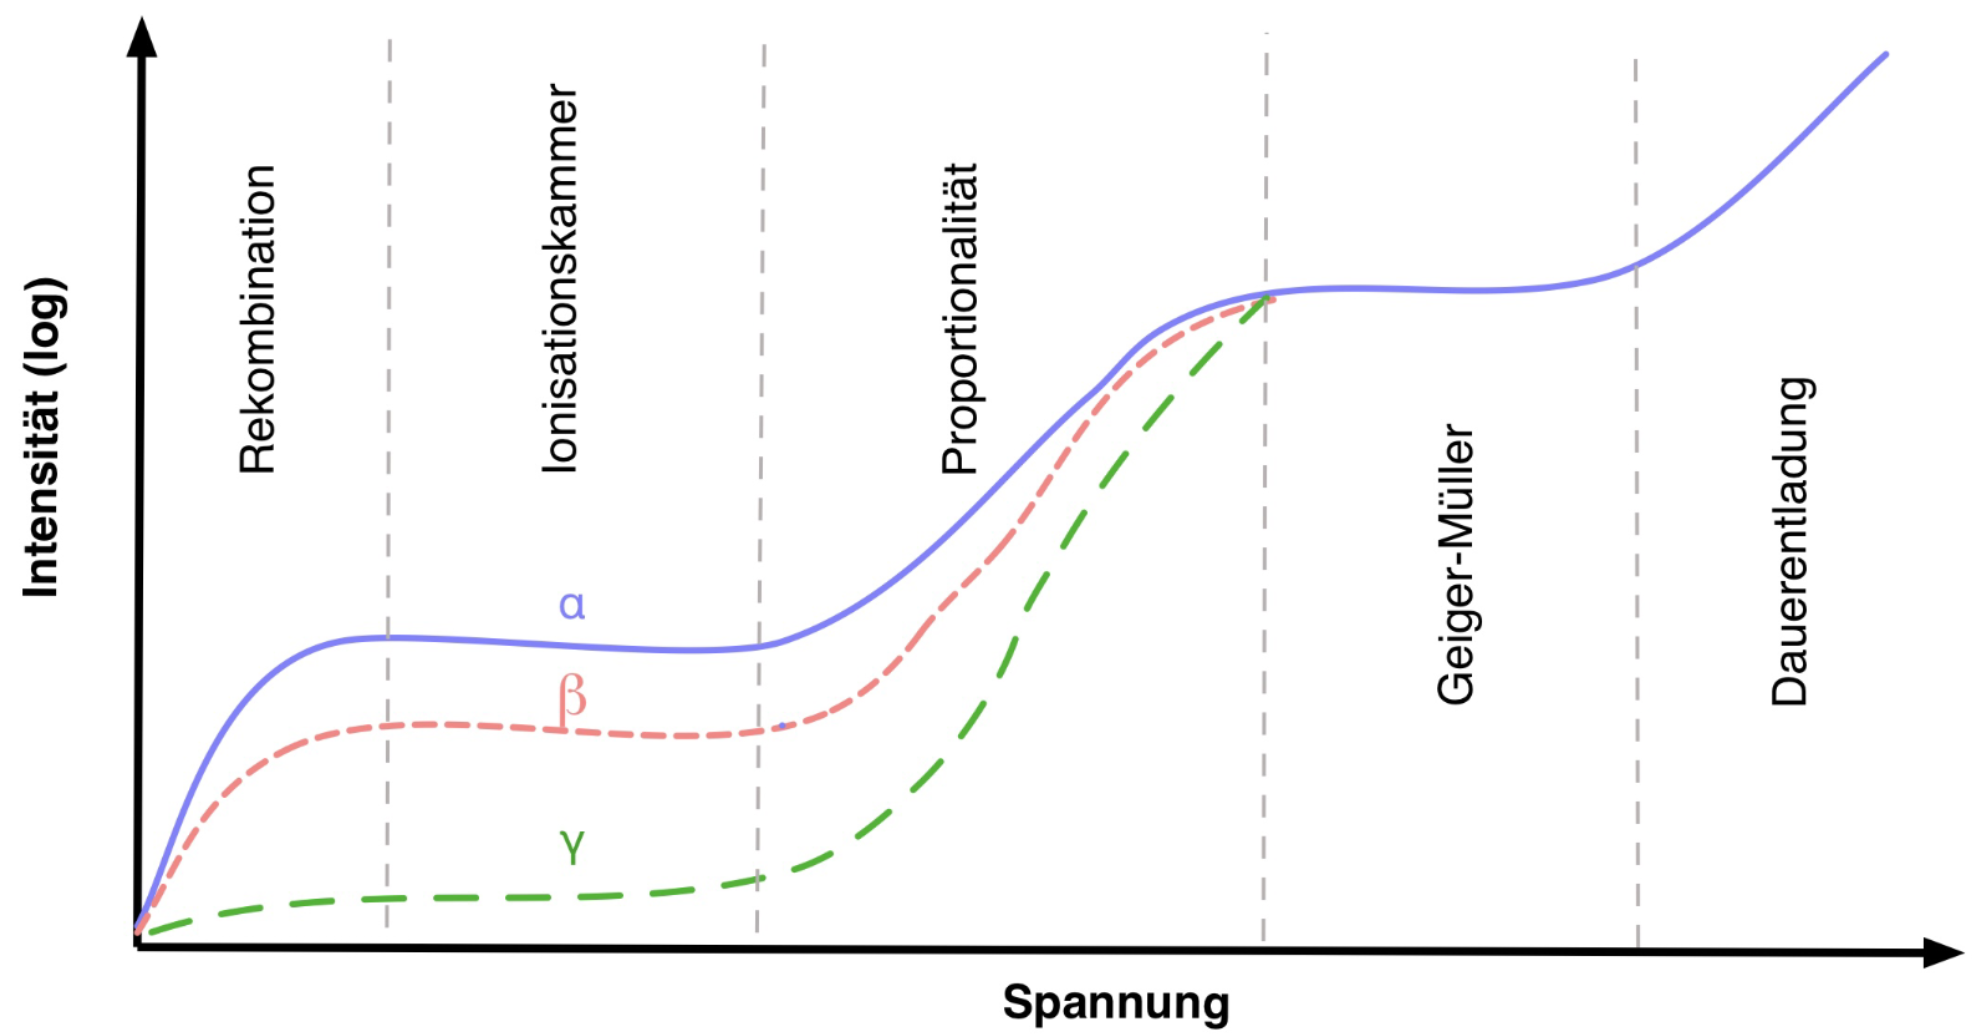
\includegraphics[width=0.5\textwidth]{img/gm-charakteristik.png}
    \caption{Charakteristische Bereiche des Geiger-Müller-Zählrohrs.\cite{V703}}
\end{figure}
Das \textbf{Detektierverhalten} des Geiger-Müller-Zählrohrs ist abhängig von der angeschlossenen Spannung.
Die Interaktion mit Strahlung lässt sich, wie in \autoref{fig:gm-charakteristik} zu sehen, in mehrere Bereiche aufteilen.
Im ersten Bereich, der Rekombination, verbinden sich Gasionen und Elektronen 
mehrheitlich bevor sie die Kathode, beziehuungsweise die Anode erreichen. 
\\
Im Bereich \textbf{Ionisationskammer} verhält sich das Zählrohr wie eine Ionisationskammer.
Es kommt zu einem vernachlässigbar geringen Menge an Rekombination.
Es werden nur Ladungen detekiert, die durch die eingehende Strahlung getrennt werden.
\\
Im \textsc{Proportionalitätsbereich} werden Ladungspaare auch durch freie Elektronen erzeugt.
Die große Feldstärke in der Nähe des Drates lößt Townsend-Lawinen aus. Dabei werden örtlich begrenzt hohe Mengen an Elektronen freigesetzt.
Abhängig von Spannung, Gasart und Gasdruck kommt es zu einer Verstärkung des Strahlungsimpulses.%?????
\\